\documentclass[10pt]{beamer}

\usepackage[frenchb]{babel}
\usepackage[T1]{fontenc}
\usepackage[utf8]{inputenc}
\usepackage{hyperref}
\usepackage{listings}
\usepackage{fancyvrb}
\usepackage{tikz}
\usepackage{framed}
\usepackage{algorithm}
\usepackage{algorithmic}
  \usepackage{amsmath,amssymb,amsthm}
  \usepackage{dsfont}\let\mathbb\mathds
\usepackage{setspace}

\usetikzlibrary{shapes.geometric}
\usetikzlibrary{shapes.arrows}
\usetikzlibrary{arrows}
\usepackage{array}

%\usetheme{Boadilla}
\usetheme{inria}
\usepackage{helvet}
\usecolortheme{dolphin}
\newcommand{\R}{\mathbb{R}}
\newcommand{\C}{\mathbb{C}}
\newcommand{\N}{\mathbb{N}}
\newcommand{\Z}{\mathbb{Z}}


\newcommand{\inriaswitchcolors}[1]{%
\pgfaliasimage{figfootline}{figfootline-#1}% !!!
\pgfaliasimage{figbackground}{figbackground-#1}% !!!
\pgfaliasimage{figbackground}{figbackground-#1}% !!!
}

%\inriaswitchcolors{pastelgreen}
\lstnewenvironment{codeC}
{ \lstset{language=C,
    otherkeywords={printf,scan}}
}
{}
\newcommand{\red}{\textcolor{red}}
\newcommand{\plus}[1]{\textcolor{orange}{\textbf{#1}}}
%\newcommand \emph
%Default size : 12.8 cm * 9.6 cm

\newenvironment<>{codeblock}[1]{%begin
  \setbeamercolor{block title}{fg=darkgray,bg=yellow}%
  \begin{block}{#1}}
  % \begin{codeC}}
  %  {\end{codeC}
{  
\end{block}}

\newenvironment<>{termblock}[1]{
    \setbeamercolor{block title}{fg=white,bg=lightgray}%
    \begin{block}{#1}}
%     \begin{Verbatim}}
{%\end{Verbatim}
\end{block}
}
%\newcommand{\output}[1]{

%%% Paramètres du cours (à régler)
%Numéro du cours
\newcommand{\nb}{1}
\setbeamertemplate{navigation symbols}{}%remove navigation symbols

\title[Renormalisation]{L'algorithme de \mbox{renormalisation}}
\subtitle{Application au Shallow-Water}
\author[J. Brajard]{julien.brajard@locean-ipsl.upmc.fr}
\institute[CLIME]{Inria CLIME}
\date{18 Septembre 2015}
\begin{document}
%%%%%%%%%%%%%%%%%%%%% SLIDES DE TITRE
\begin{frame}
\titlepage
\end{frame}
%%%%%%%%%%%%%%%%%%%%%
\begin{frame}
\frametitle{Contexte de cette présentation}

\begin {block}{}
La méthode de renormalisation est une méthode proposé dans~\cite{issartel2007} pour la détection de source dans la dispersion atmosphérique.
\end{block}
\bibliographystyle{apalike} 
\bibliography{bib-assim.bib}
\end{frame}

%%%%%%%%%%%%%%%%%%%%%%%%%%%%%%%%%%%%%%%%

\begin{frame}[t]
\setbeamercovered{transparent=50}
\frametitle{Objectif général}
\begin{columns}
\column{.5\textwidth}
\uncover<1-4>{
\begin{block}{Détermination de sources}
\begin{itemize}[<visible@+->]
\item  Existence d'une \plus{source} de traceur inconnue $\sigma(x,y,z,t)$.\\
\item  Un \plus{modèle} $M$ linéaire d'advection/diffusion permet de relier la source à la concentration de ce traceur en tout point : $\chi(x,y,z,t) = M.\sigma(x,y,z,t)$.\\
\item  On dispose de $m$ \plus{observations} ponctuelles de concentration $\mu_i=<\pi_i,\chi>$.\\
\end{itemize}
\visible<4-> {\textbf {\red{Objectif :} Retrouver le \textit{meilleur} $\sigma$ sachant $\mu_i$ et $M$.}}
\end{block}
}
\column{.5\textwidth}

\only<5->{
\begin{block}{Conditions initiales}
\begin{itemize}
\item Existence d'une \plus{hauteur} d'eau initiale inconnue $h(x,y,0)$.\\
\item Un \plus{modèle} linéaire permet d'estimer la hauteur à tout moment : $h(x,y,t)=M.h(x,y,0)$.\\
\item On dispose de $m$ \plus{observations} ponctuelle de hauteur réparties dans le temps $\mu_i = <\pi_i,h>$.\\
\end{itemize}
\visible<6-> {\textbf{\red{Objectif :} Retrouver le \textit{meilleur} champs de hauteur initial $h(x,y,0)$ sachant $\mu_i$ et $M$.}}
\end{block}
}
\end{columns}
\end{frame}


\begin{frame}
\setbeamercovered{transparent=0}
\frametitle{Formalisme du problème discrétisé}
\begin{columns}
\column{.4\textwidth}
\begin{block}{Le modèle direct}
\begin{itemize}
\item $\sigma = h(x_j,y_j,0)$ de dimension $p$\\
\item $\chi = h(x_j,y_j,t_j)$ de dimension $n$\\
\item Le modèle $M \in \R^{n\times p}$.\\
\end{itemize}
On a alors :
\begin{equation}
\chi = M.\sigma \nonumber
\end{equation}
\end{block}
\column{.6\textwidth}
\begin{block}<2->{Le modèle adjoint}
\begin{itemize}
\item $\pi_i \in \R^n$ ($i=1..m$) est l'opérateur d'observation.\\
\item $\mu_i \in \R$ ($i=1..m$) est la ième observations définie par :
$
\mu_i = <\pi_i,\chi>
$
\end{itemize}
%\begin{spacing}{0.9}
On peut donc écrire :
\begin{eqnarray*}
\mu_i & = & <\pi_i,\chi> \\
      & = & <\pi_i,M.\sigma>\\
      & = & <M^*.\pi_i,\sigma>\\
      & = & <r_i,\sigma>
\end{eqnarray*} 
$r_i$ est appelé adjoint associé à la mesure $\mu_i$.

%\end{spacing}
\end{block}
\end{columns}
\end{frame}

\begin{frame}
\frametitle{Equation à résoudre}
Si on note :
$$
\mu=
\begin{pmatrix}
\mu_1 \\ 
\vdots\\ 
\mu_m
\end{pmatrix}
$$


$$
R=
\begin{pmatrix}
{}^\top{r_1}\\
 \vdots\\ 
{}^\top{r_m}
\end{pmatrix}
$$
\begin{alertblock}{Système à résoudre}
$$
R.\sigma = \mu
$$
\end{alertblock}
\end{frame}

%%%%%%%%%%%%%%%%%%%%%%%%%%%%%%%%%

\begin{frame}
\frametitle{Le modèle shallow-water}
\begin{eqnarray*}
\partial_tu & = & -g^*.\partial_xh + f . v - \gamma . u \nonumber \\
\partial_tv & = & -g^*.\partial_yh - f . u - \gamma . v \label{shal-lin}\\
\partial_th & = & - H.(\partial_xu + \partial_yv) \nonumber
\end{eqnarray*}

\begin{block}{paramètres utilisés : }
\centering
\begin{tabular}{rcll}
%$\Delta t$ & = & $1500 s$ \\
%$\Delta x$ & = & $5000 m$ \\
%$\Delta y$ & = & $5000 m$ \\
$f$ & = & $0.0001 s^{-1}$& (paramètre de coriolis)\\
$g^*$& = & $0.01 m.s^{-2}$& (gravité réduite)\\
$\gamma$& = & $0.00001s^{-1}$& (dissipation)\\
%$\alpha$& = & $0.15$\\
$H$& = & $100 m$ & (Hauteur moyenne)\\
\end{tabular}
\end{block}

\end{frame}

%%%%%%%%%%%%%%%%%%%
\begin{frame}[fragile]
\frametitle{Modèle numérique}
\begin{itemize}
\item \textbf{Schéma spatial} : différences finies centrées sur une grille C d'Arakawa
\begin{verbatim}
h(i,j)  --  u(i,j) -- h(i+1,j)
   |          |
v(i,j)  --  z(i,j)
   |
h(i,j-1) 
\end{verbatim}


\item \textbf{Schéma temporel} : Schéma leap-frog (saute-mouton) d'ordre 2 avec filtre d'Asselin

\begin{equation}
\hat{x}_{ijt}  = x_{ijt} + \alpha(\hat{x}_{ijt-1} - 2 x_{ijt} + x_{ijt+1})\nonumber
\end{equation}
avec $\hat{x}$ désignant la valeur filtrée de la grandeur physique $x=h$,$u$ ou $v$.\\


\end{itemize}
\end{frame}




%%%%%%%%%%%%%%%%%%%%%%%%%%
\begin{frame}
\frametitle{Configuration du modèle}

\begin{columns}

\column{6cm}
\onslide<1->{
\begin{figure}
\centering

\begin{tikzpicture} [
    auto,
      block/.style    = { rectangle, draw=blue, thick, 
                        fill=blue!20, text width=1.3cm, text centered,
                        rounded corners, minimum height=2em,scale=0.8 },
    line/.style     = { draw, thick, ->, shorten >=2pt,text width=4cm},
    etiq/.style = {scale=0.8,midway,xshift=+4mm,right},
    node distance=1.5cm,
  ]
\node (H0) [block]{$h_0$};
\node (Init) [block,below of = H0]{$h_0$,$u_0$,$v_0$};
\node (t1) [block,below of = Init]{$h_1$,$u_1$,$v_1$};
\node (buf1) [below of = t1,yshift=+4mm]{...};
\node (tn) [block,below of = buf1,yshift=+4mm]{$h_t$,$u_t$,$v_t$};
\node (buf2) [below of = tn,yshift=+4mm]{...};
\node (obs) [block,below of =buf2,yshift=+4mm]{$h_{obs}$};

\begin{scope}[every path/.style=line]
\path (H0) -- node[etiq] {Equilibre géostrophique} (Init);
\path (Init) -- node[etiq] {Modèle (Euler)} (t1);
\path (t1) -- node[etiq] {Modèle (leap-frog)}(buf1);
%\path (buf1) -- node[etiq] {Modèle (leap-frog)}(tn);
%\path (tn) -- (buf2);
\path (buf2) -- node[etiq] {Echantillonnage}(obs);
\end{scope}

\end{tikzpicture}

\end{figure}
}
\column{6cm}
\onslide<2->{
\begin{block}{Paramètres}
\centering
\begin{tabular}{rcl}
$\Delta t$ & = & $1500 s$ \\
$\Delta x$ & = & $5000 m$ \\
$\Delta y$ & = & $5000 m$ \\
$\alpha$& = & $0.15$\\
\end{tabular}
\end {block}
}
\end{columns}

\end{frame}


%%%%%%%%%%%%%%%%%%%%%%%%%%%%%%%%

\begin{frame}
\frametitle{Exemple de simulation}
\begin{columns}
\column{.5\textwidth}
\begin{figure}
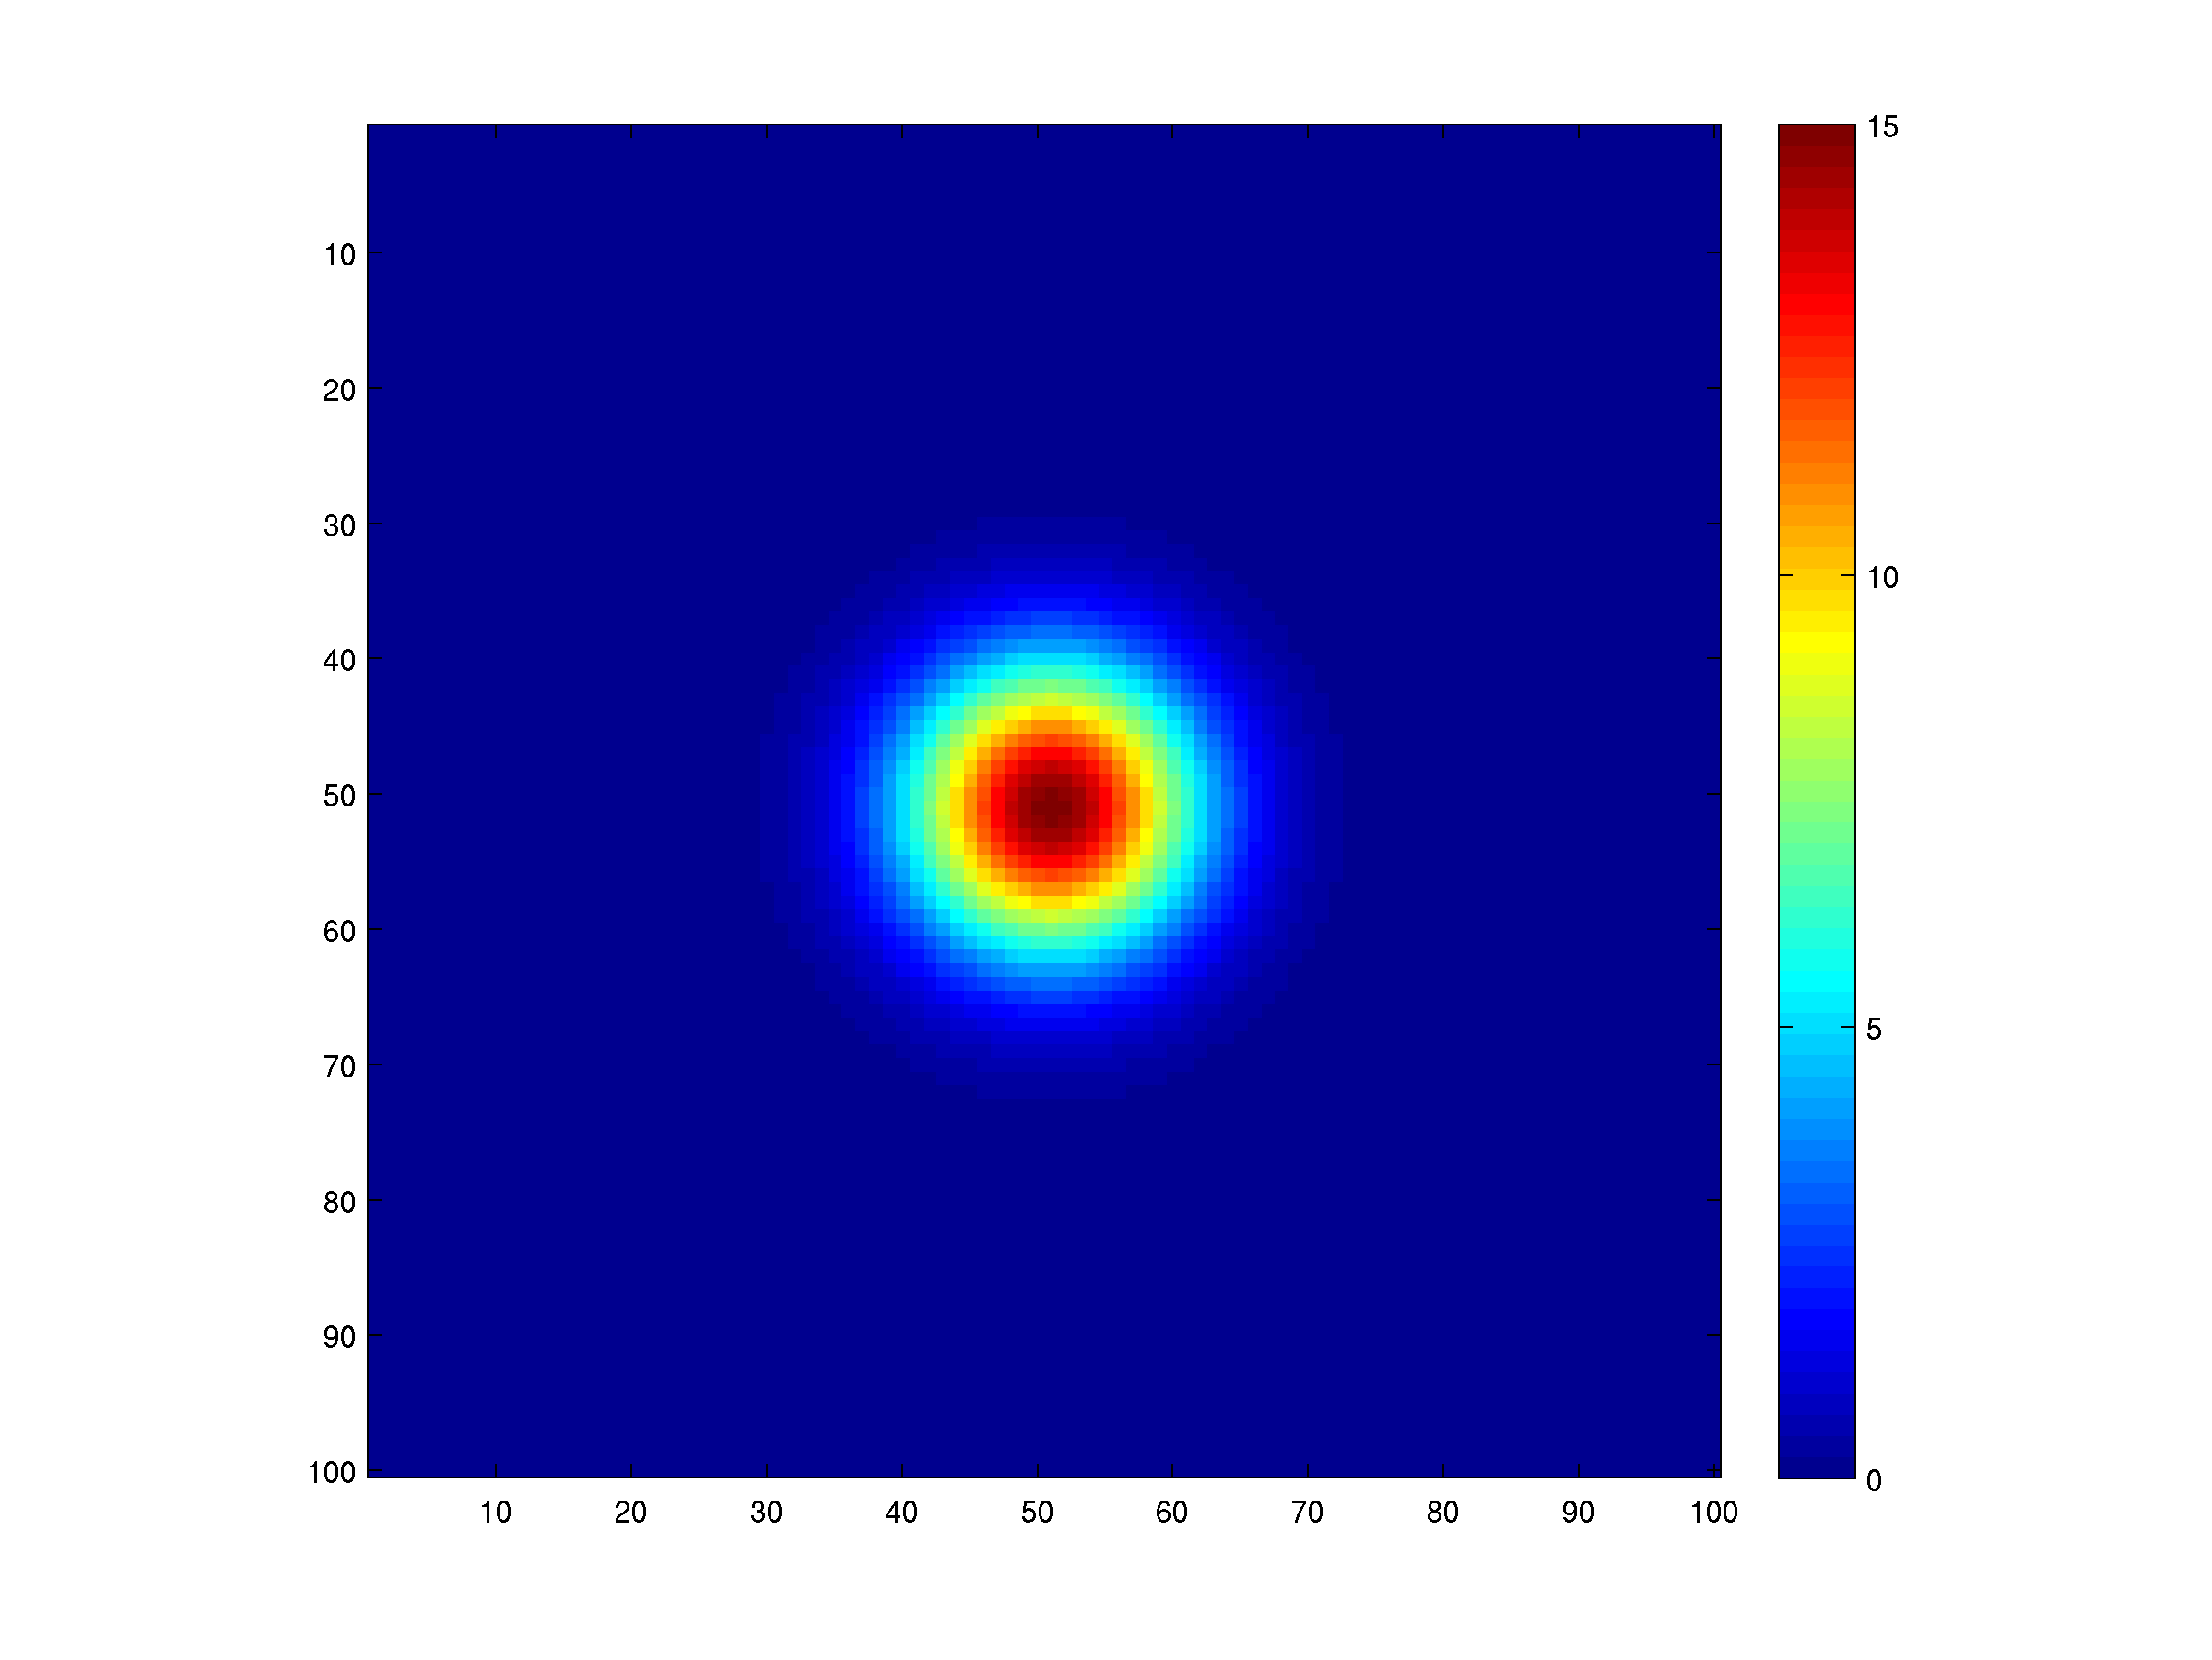
\includegraphics[scale=0.3]{./fig/fig1.png}
\caption{Hauteur à t=0}
\end{figure}
\column{.5\textwidth}
\begin{figure}
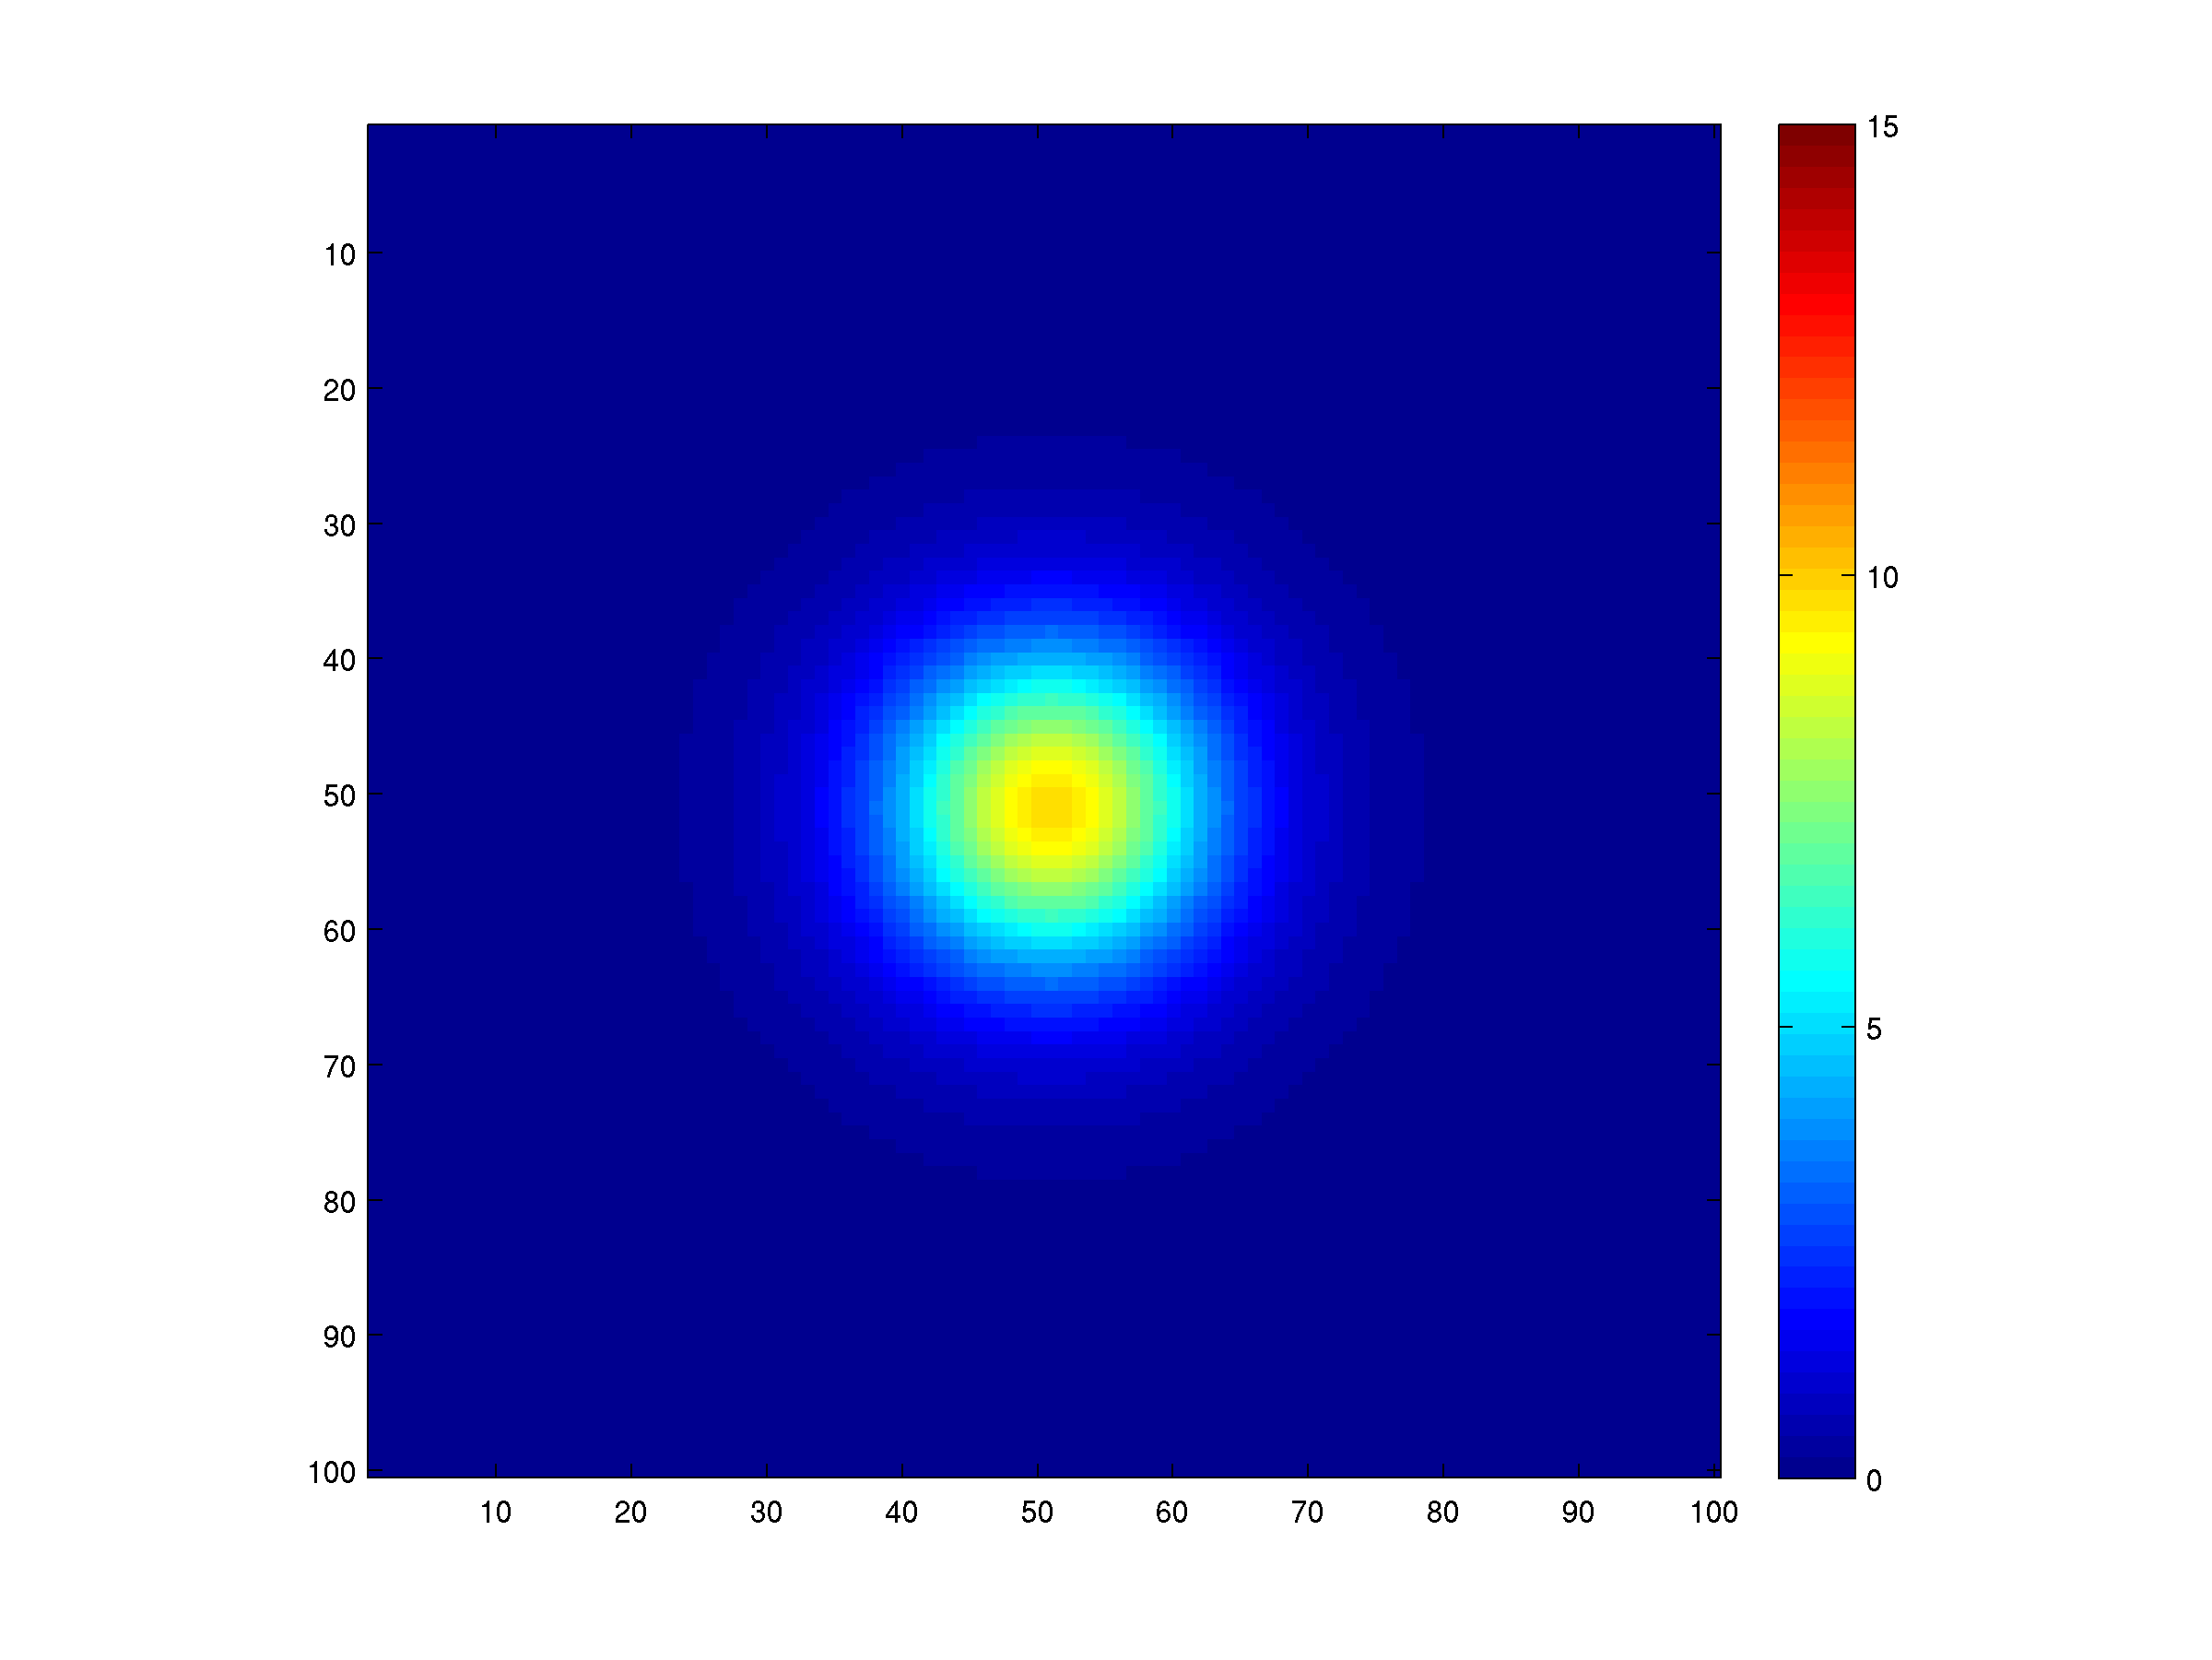
\includegraphics[scale=0.3]{./fig/fig2.png}
\caption{Hauteur à t=300pdt}
\end{figure}
\end{columns}
\end{frame}

\begin{frame}
\frametitle{Evolution temporelle}
\begin{figure}
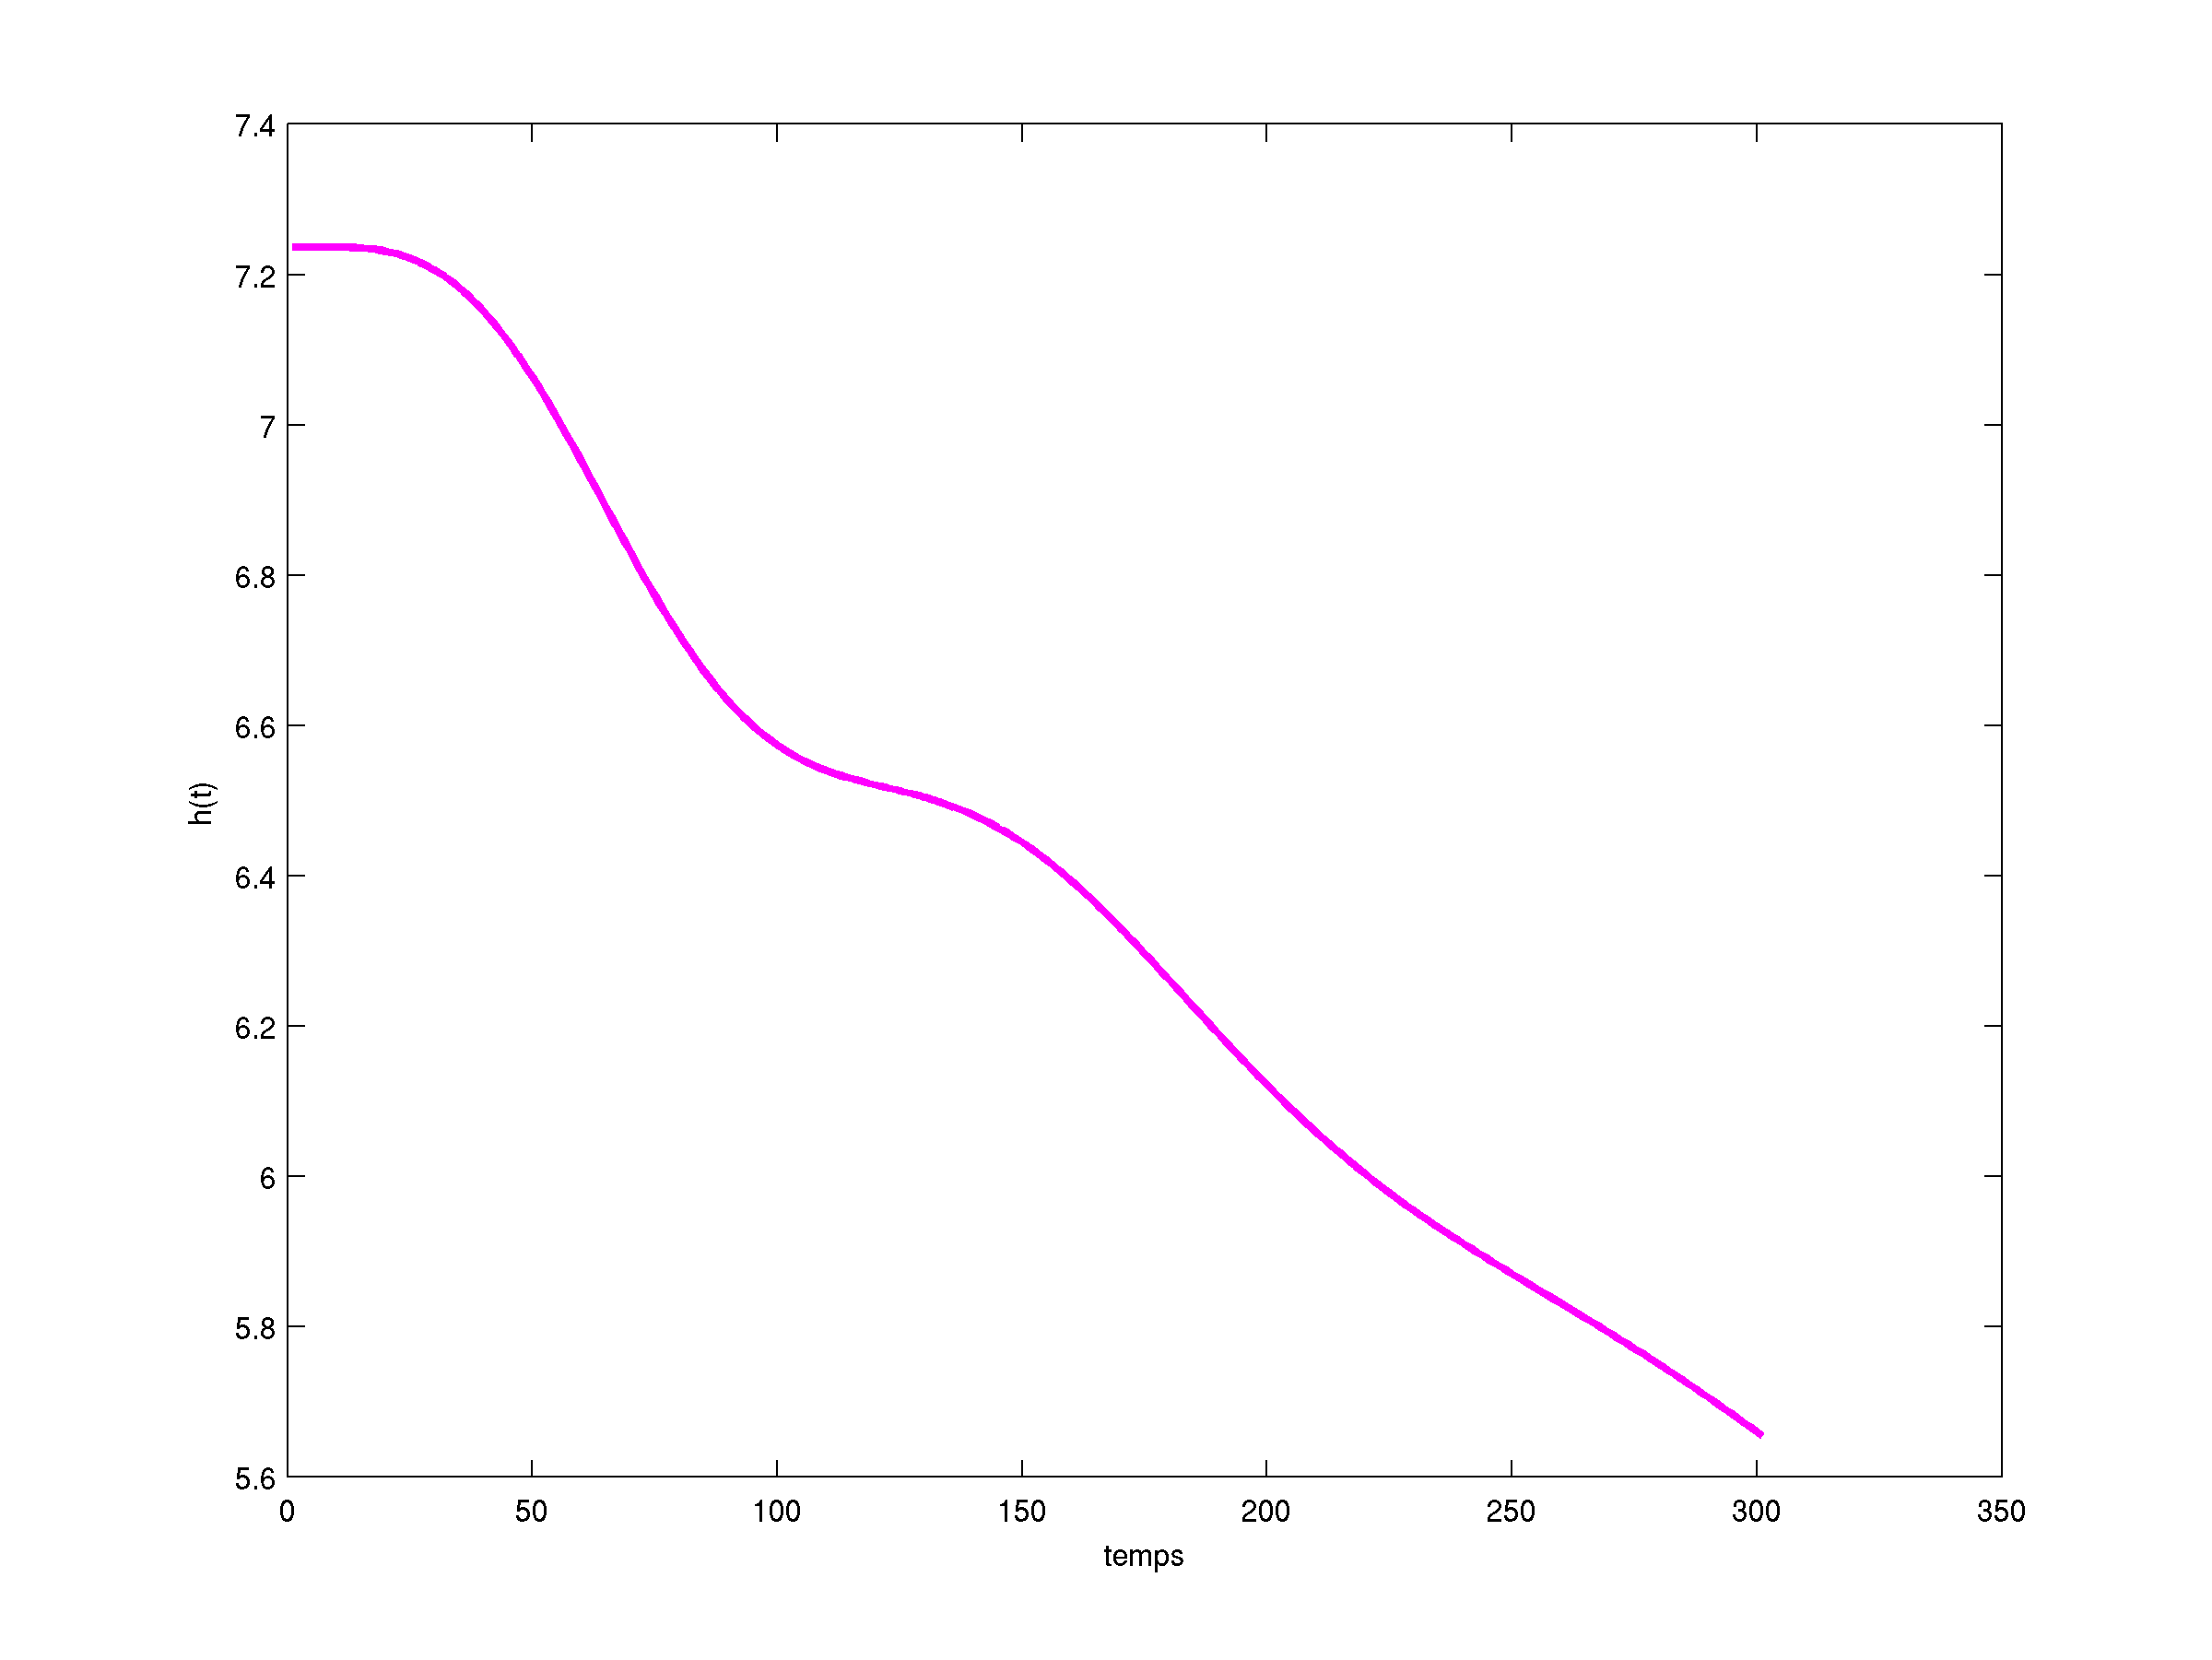
\includegraphics[scale=0.4]{./fig/fig3.png}
\caption{Hauteur du point de coordonné (60,50) }

\end{figure}

\end{frame}

\begin{frame}
\frametitle{La fonction adjointe}
\framesubtitle{associée au point (50,50)}
\begin{figure}
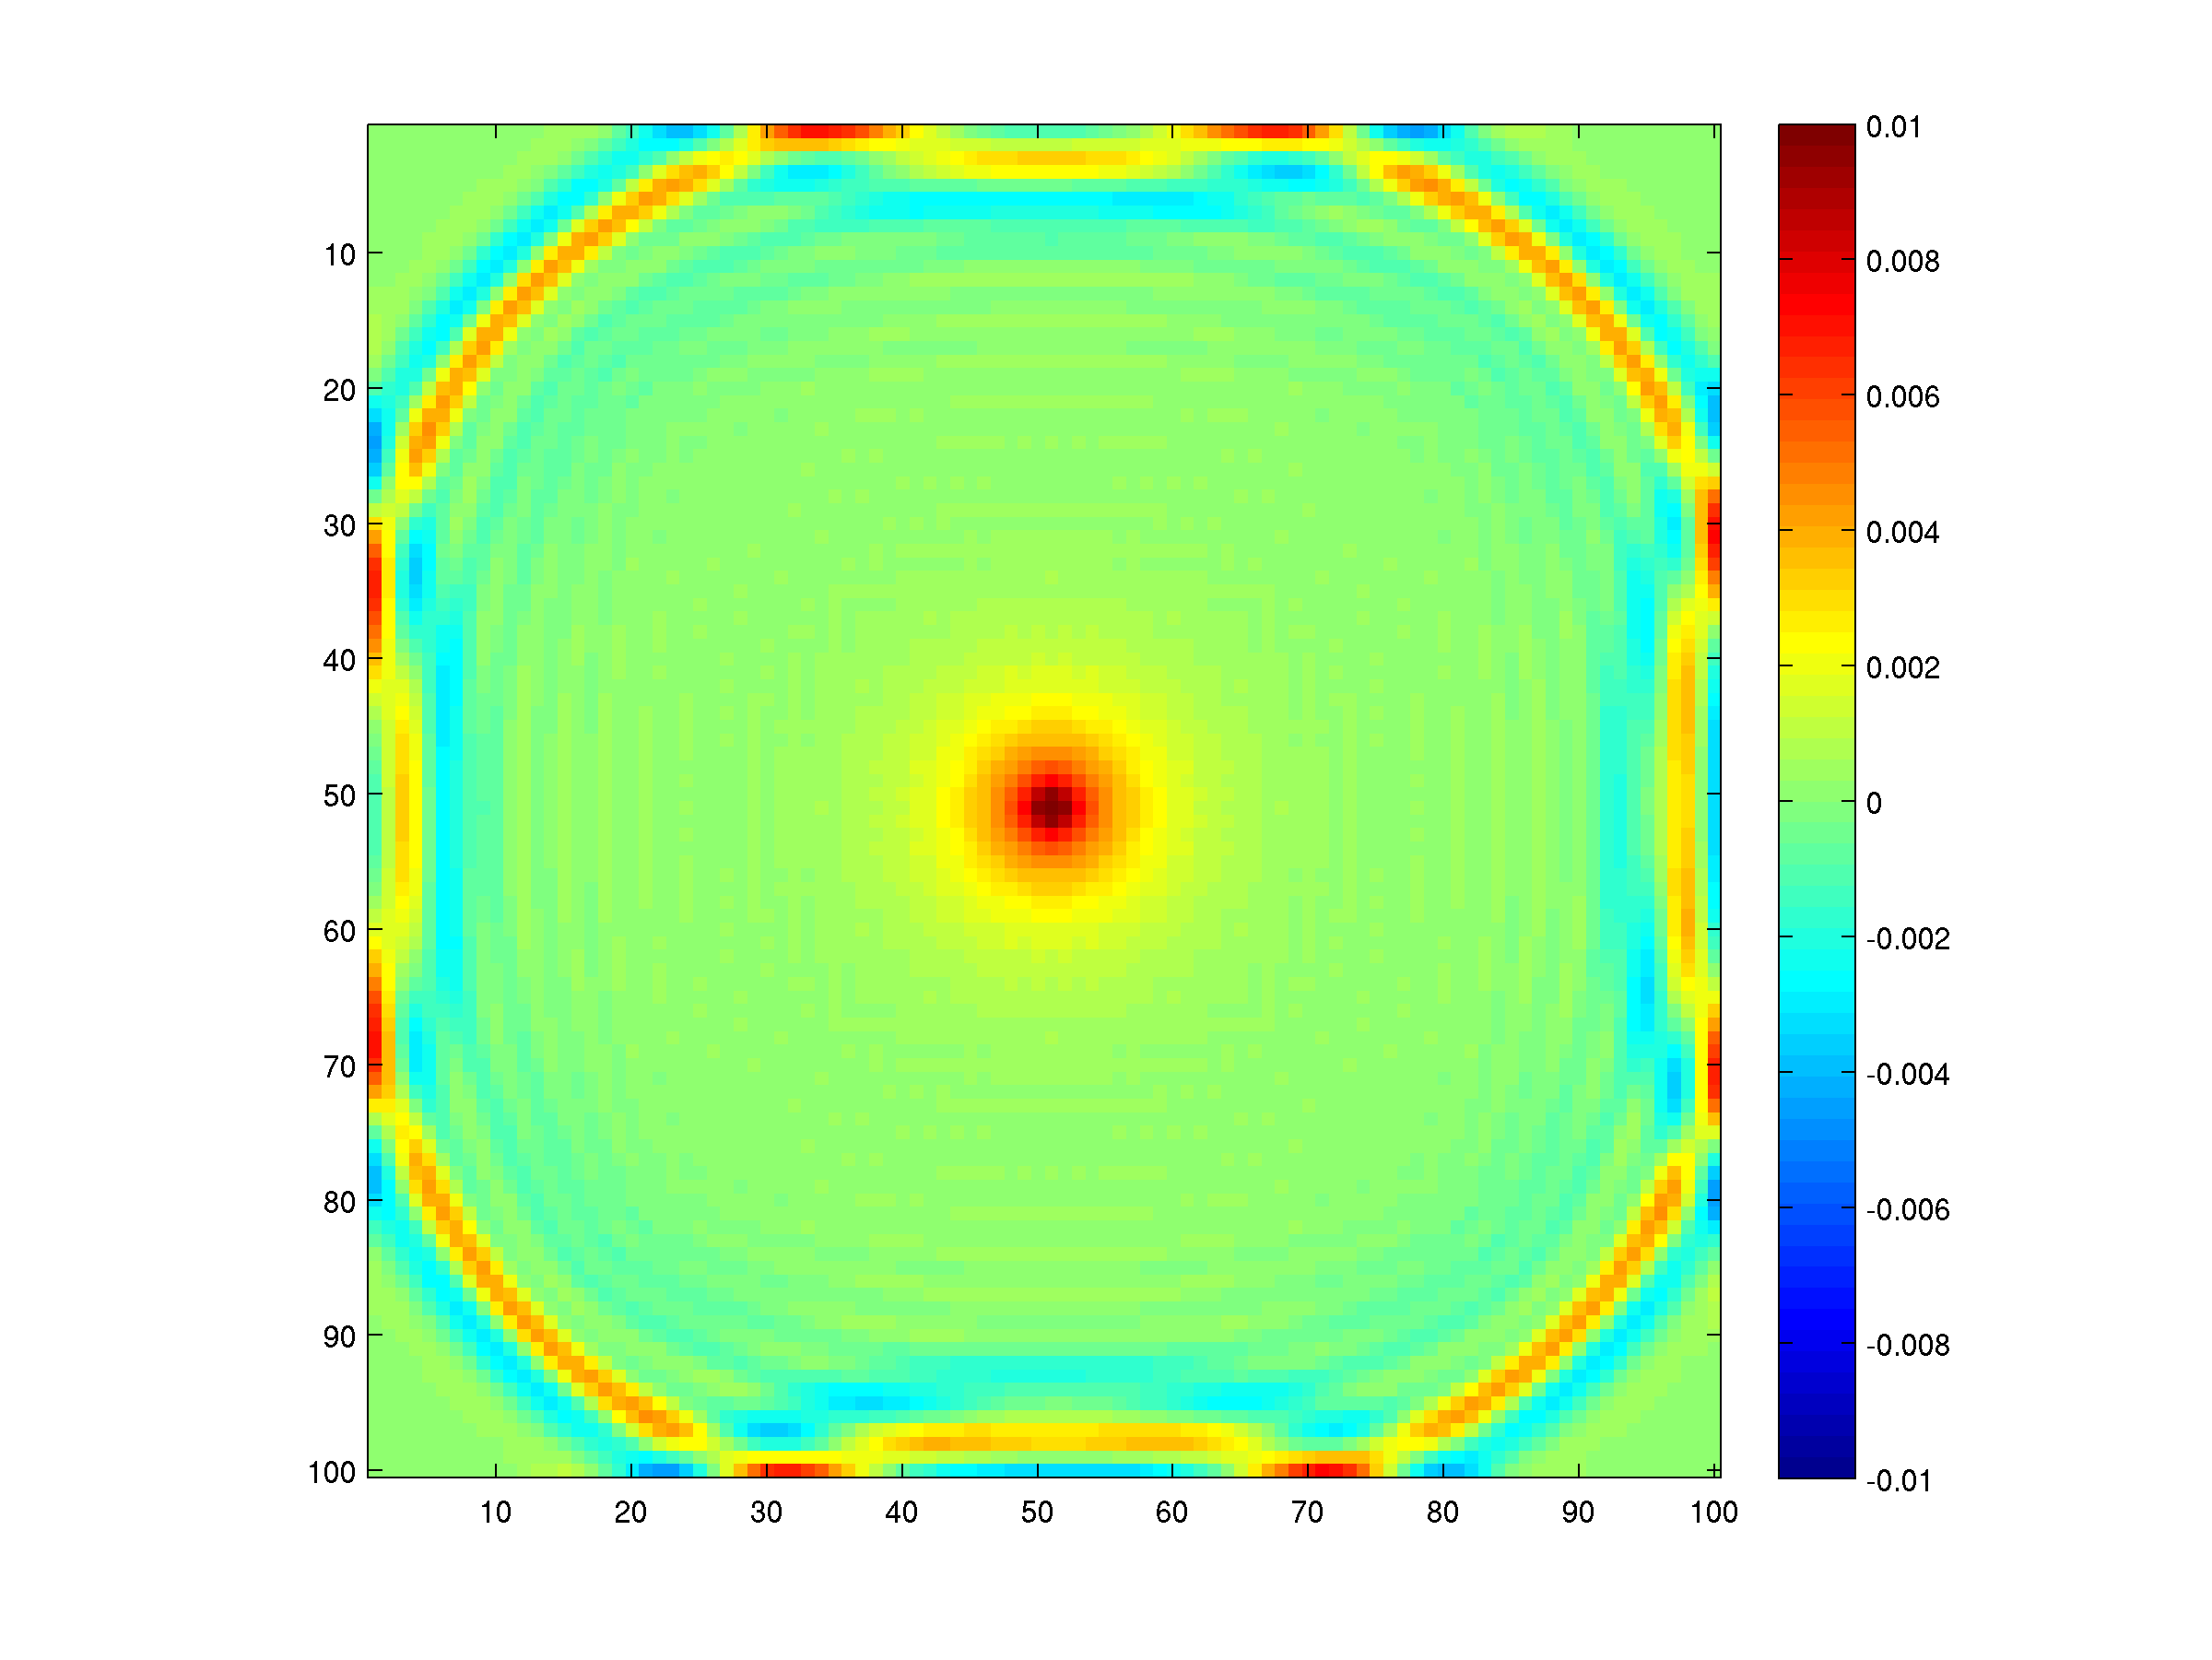
\includegraphics[scale=0.4]{./fig/fig4.png}
\end{figure}
\end{frame}

\begin{frame}
\frametitle{Solution naïve au problème}
\begin{block}{Système à résoudre}
$$
R.\sigma = \mu
$$
\end{block}

\begin{alertblock}{Solution par la pseudo-inverse (ou Moore-Penrose)}
$$
\sigma^*={}^\top{R}.(R.{}^\top{R})^{-1}.\mu
$$
\end{alertblock}
Propriété : Parmi toutes les solutions possibles, $\sigma^*$ \plus{minimise} $\|\sigma \|$.
\end{frame}

\begin{frame}
\frametitle{Solution de la pseudo-inverse}
\framesubtitle{4 observations}
\begin{figure}
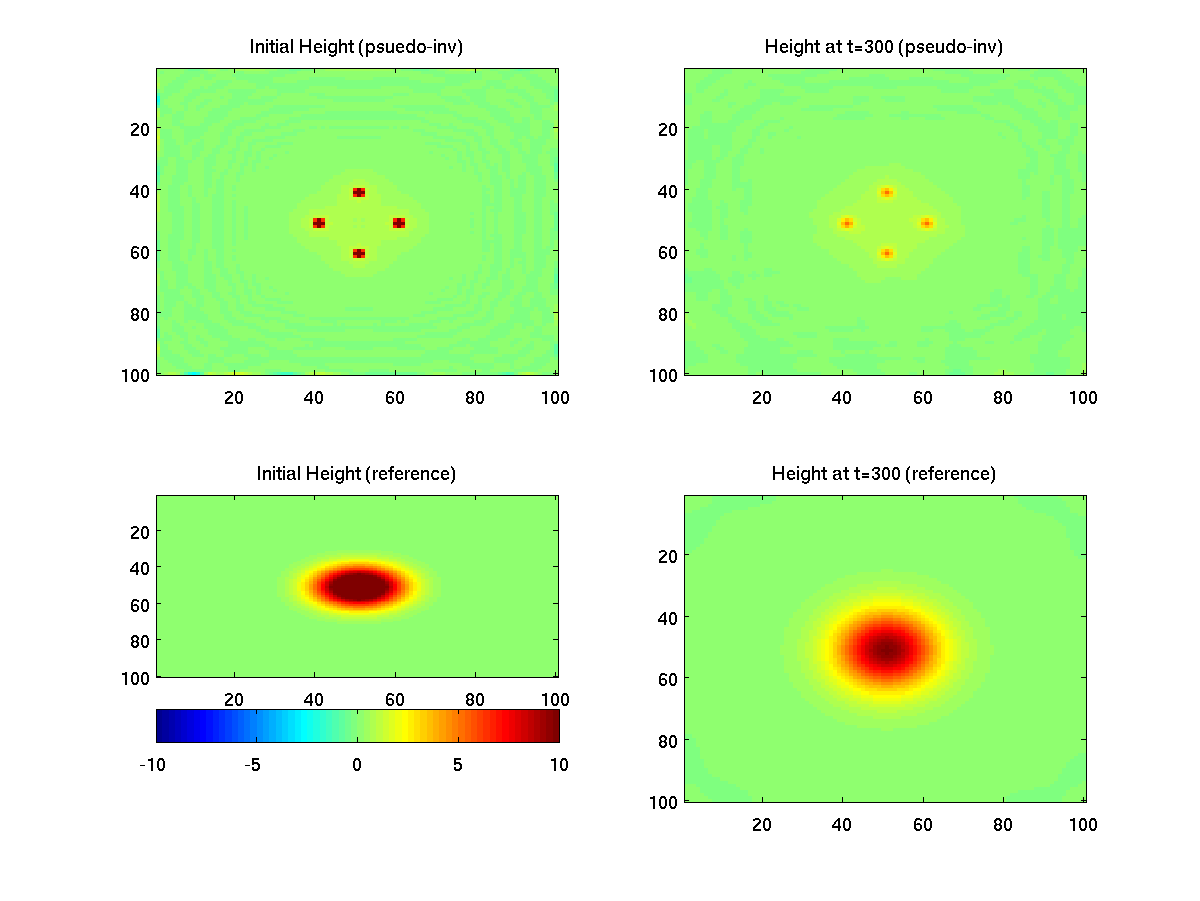
\includegraphics[scale=0.5]{./fig/4obs/pseudoinv-sol.png}
\end{figure}
\end{frame}

\begin{frame}
\frametitle{La renormalisation}
Minimal au sens de la norme F
\end{frame}

\begin{frame}
\frametitle{Détermination de $F^{opt}$}
Propriété dans le cas d'une source ponctuelle.
\end{frame}

\begin{frame}
\frametitle{Expérience avec le shallow-water}
4 points
montrer F, parler de visibilité
\end{frame}

\begin{frame}
\frametitle{Solution obtenue avec la pseudo inverse}
\end{frame}

\begin{frame}
\frametitle{Autre exemple}
\end{frame}


\begin{frame}
\frametitle{Les équations du shallow-water linéaire}
\begin{eqnarray*}
\partial_tu & = & -g^*.\partial_xh + f . v - \gamma . u \nonumber \\
\partial_tv & = & -g^*.\partial_yh - f . u - \gamma . v \label{shal-lin}\\
\partial_th & = & - H.(\partial_xu + \partial_yv) \nonumber
\end{eqnarray*}

\begin{block}{paramètres utilisés : }
\centering
\begin{tabular}{rcll}
%$\Delta t$ & = & $1500 s$ \\
%$\Delta x$ & = & $5000 m$ \\
%$\Delta y$ & = & $5000 m$ \\
$f$ & = & $0.0001 s^{-1}$& (paramètre de coriolis)\\
$g^*$& = & $0.01 m.s^{-2}$& (gravité réduite)\\
$\gamma$& = & $0.00001s^{-1}$& (dissipation)\\
%$\alpha$& = & $0.15$\\
$H$& = & $100 m$ & (Hauteur moyenne)\\
\end{tabular}
\end{block}
\end{frame}


\begin{frame}
\frametitle{Résolution du système}
\begin{block}{}
\begin{equation}
h_0 = \mu^T H_f^{-1} R_f \nonumber
\end{equation}
où $\mu = h_{hobs}$, et $H_f$, $R_f$ sont définis par la méthode de renormalisation.
\end{block}
\begin{itemize}
\item Si $f=1$, on calcule exactement la solution de la pseudo-inverse,\\
\item si $f$ est tel que $R_f^T H_f^{-1} R_f \equiv 1$, on calcule la solution renormalisée.
\end{itemize}
\end{frame}

%%%%%%%%%%%%%%%%%%%%%%%%
\begin{frame}
\frametitle{Mise en oeuvre technique}
\begin{itemize}
\item Les fonction adjointes (lignes de $R$) sont calculées via le code généré par YAO.\\
\item La méthode de renormalisation est implémentée dans le code YAO à l'aide de la bibliothèque d'algèbre linéaire Seldon\footnote{\url{http://seldon.sourceforge.net/}} interfacée avec Blas et Lapack.\\
\end{itemize}
\end{frame}

%%%%%%%%%%%%%%%%%%%%%%%%

\begin{frame}
\frametitle{Première expérience (4 observartions)}
\begin{figure}
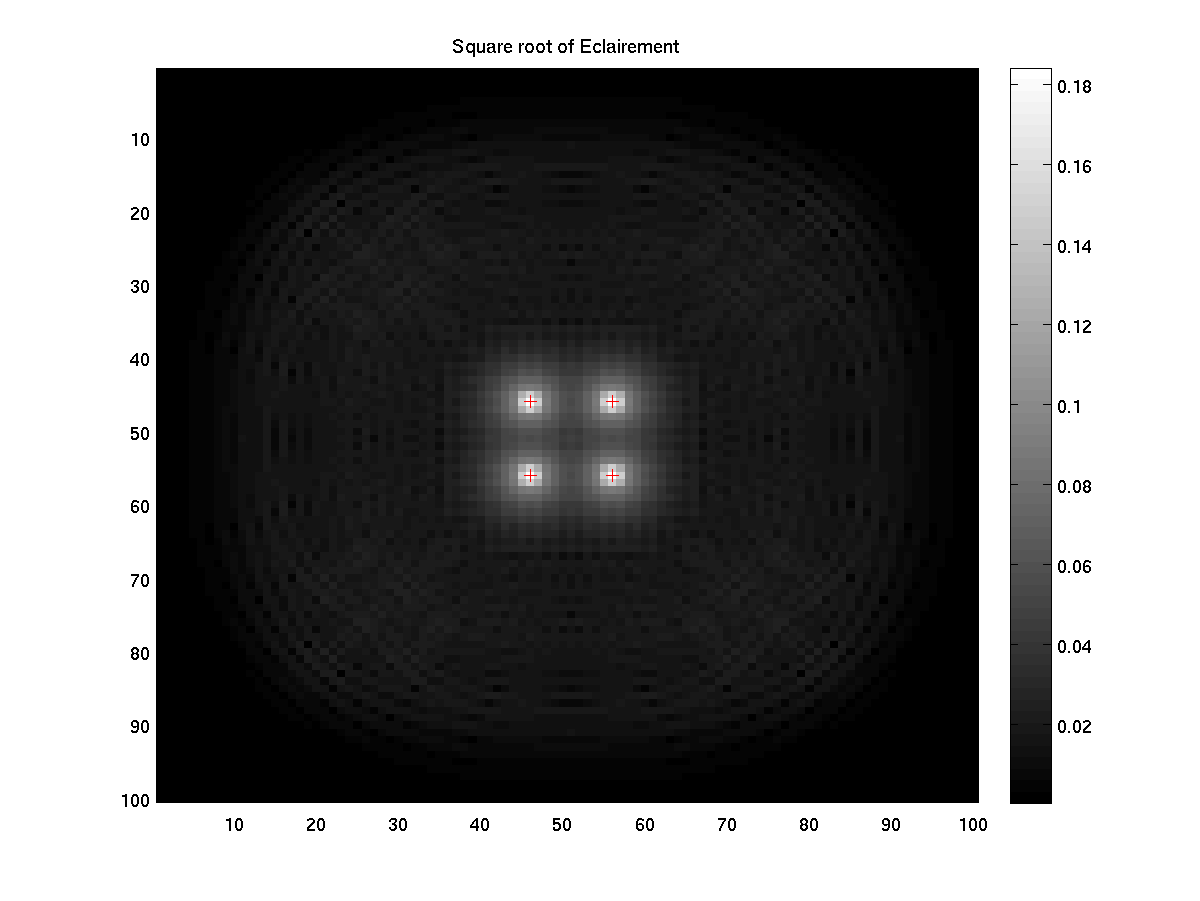
\includegraphics[scale=0.4]{./fig/4obs/eclairement.png}
\caption{Fonction d'Eclairement (en racine carré) et position des observations}
\end{figure}
\end{frame}

\begin{frame}
\frametitle{Solution de la pseudo-inverse}
\begin{figure}
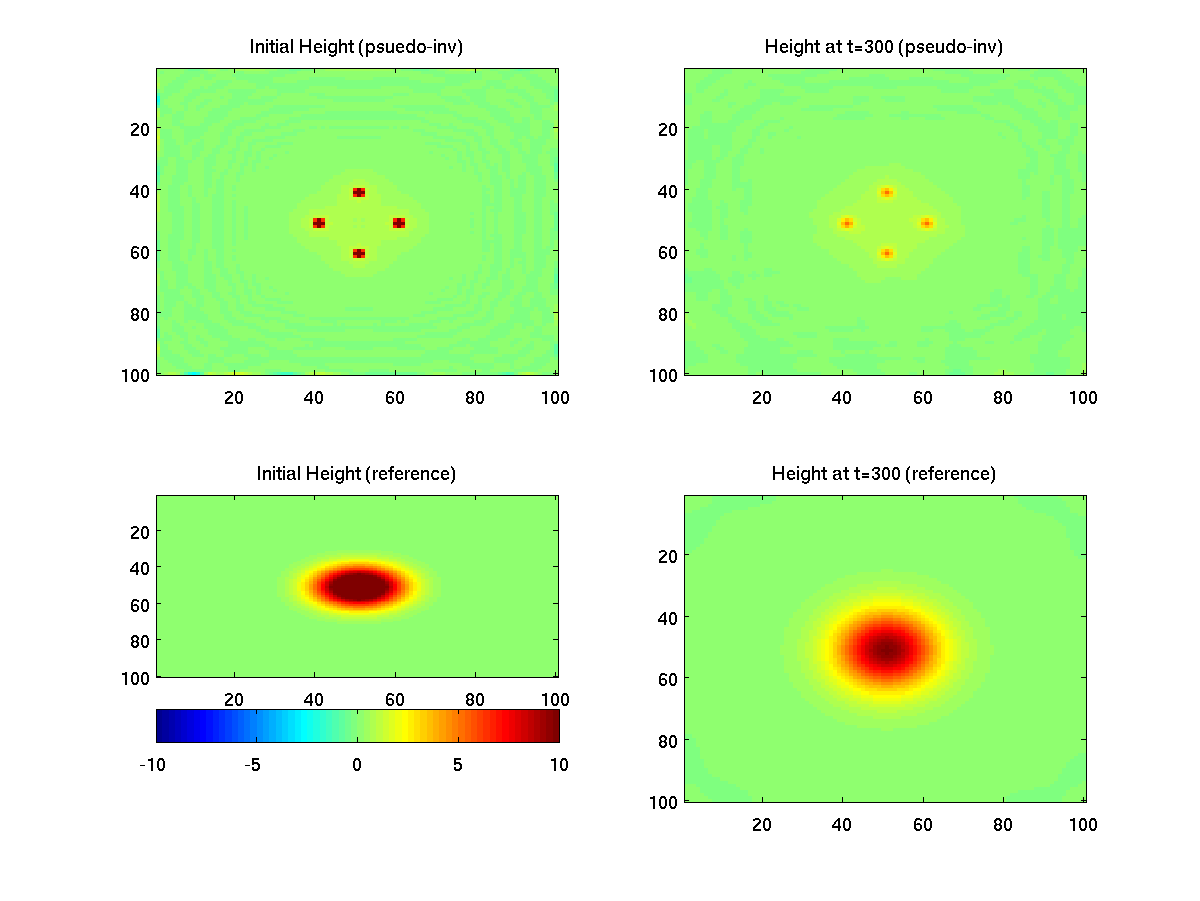
\includegraphics[scale=0.55]{./fig/4obs/pseudoinv-sol.png}
\end{figure}
\end{frame}

\begin{frame}
\frametitle{Solution par renormalisation}
\begin{figure}
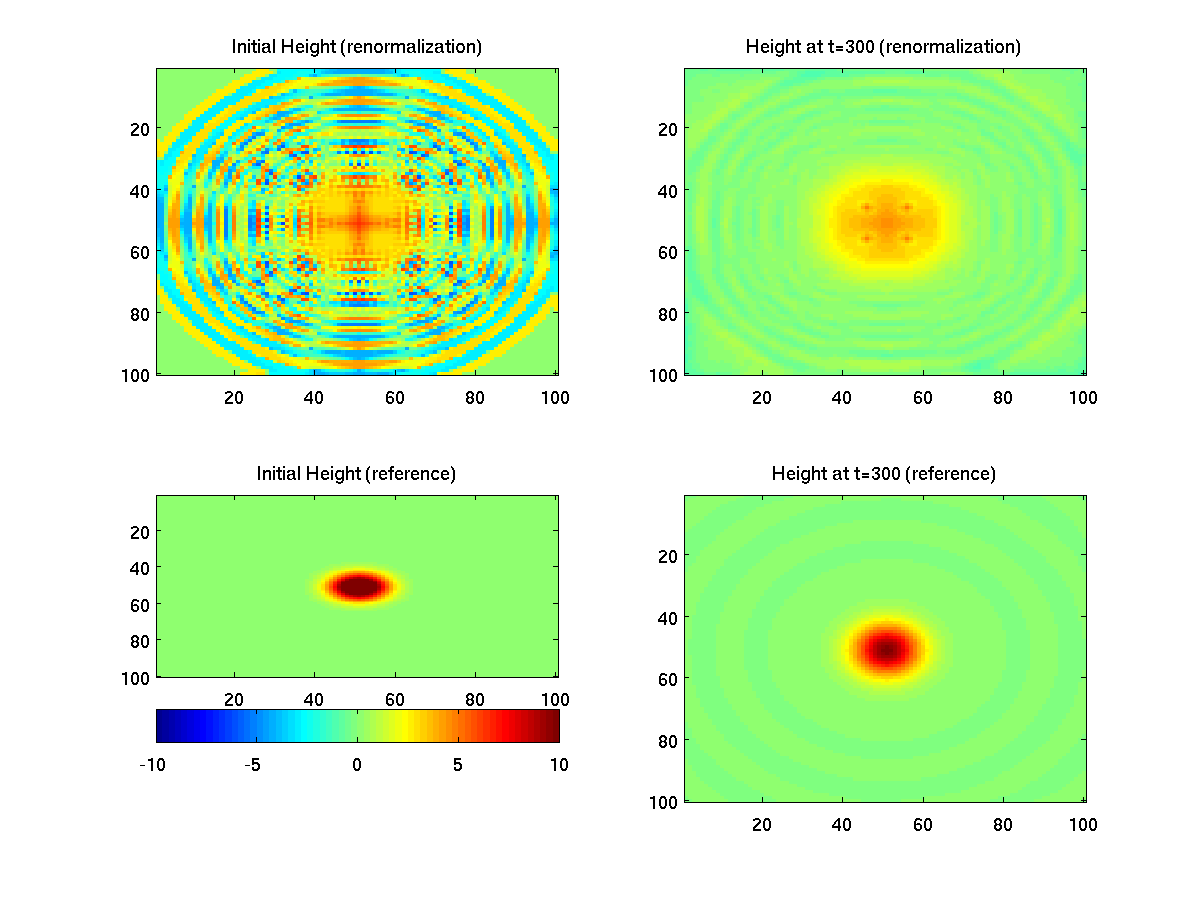
\includegraphics[scale=0.55]{./fig/4obs/renorm-sol.png}
\end{figure}
\end{frame}

\begin{frame}
\frametitle{Solutions dans le temps}
\begin{figure}
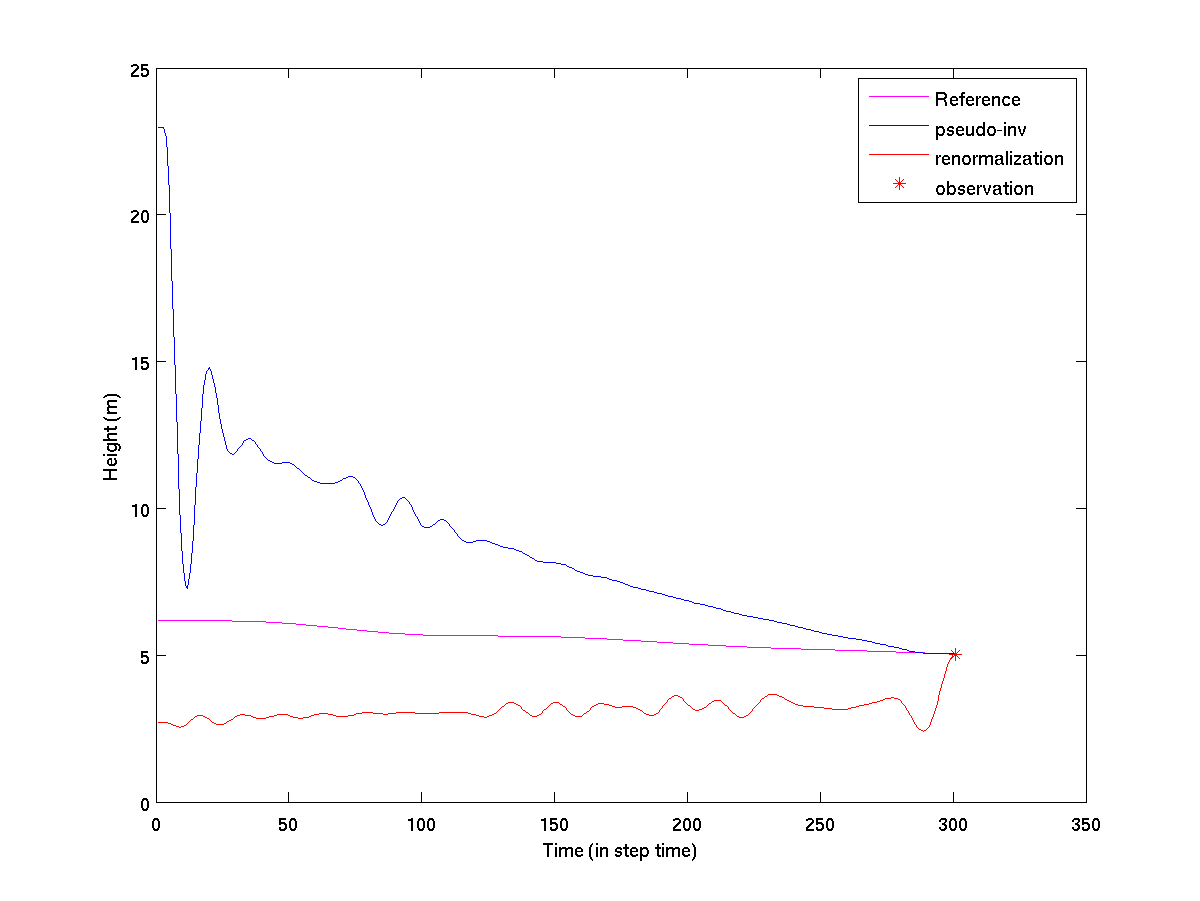
\includegraphics[scale=0.55]{./fig/4obs/compare_sol.png}
\end{figure}
\end{frame}

\begin{frame}
\frametitle{Autre expérience (121 observations)}
\begin{figure}
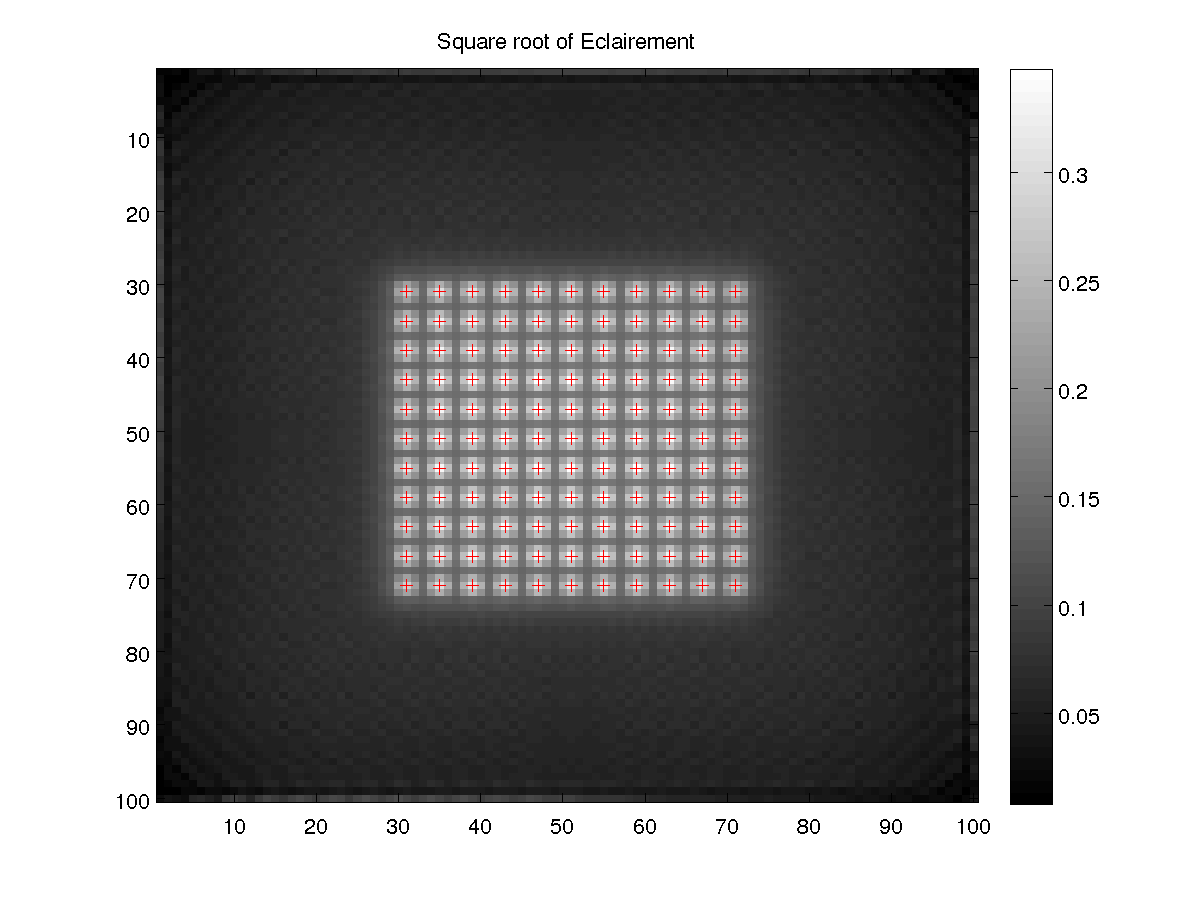
\includegraphics[scale=0.4]{./fig/121obs/eclairement.png}
\caption{Fonction d'Eclairement (en racine carré) et position des observations}
\end{figure}
\end{frame}

\begin{frame}
\frametitle{Solution de la pseudo-inverse}
\begin{figure}
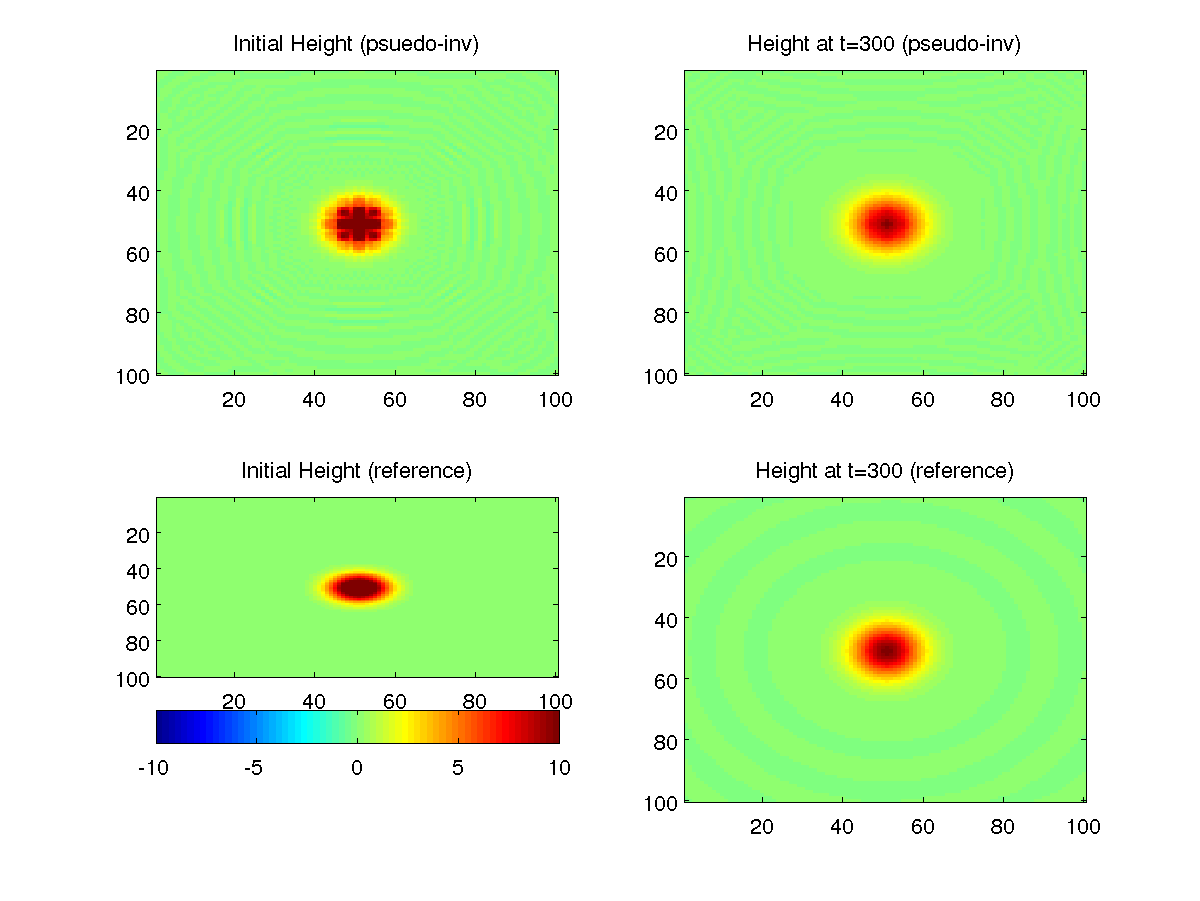
\includegraphics[scale=0.55]{./fig/121obs/pseudoinv-sol.png}
\end{figure}
\end{frame}

\begin{frame}
\frametitle{Solution par renormalisation}
\begin{figure}
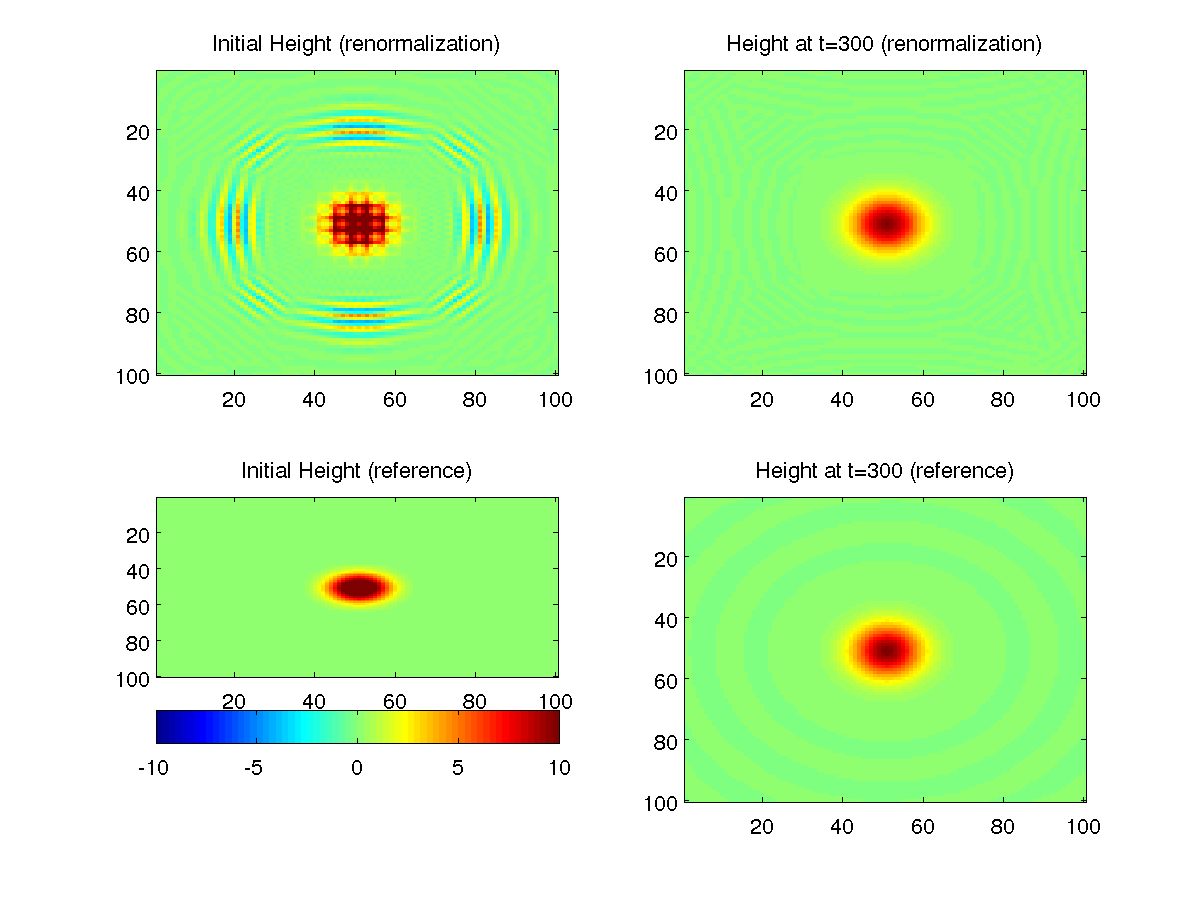
\includegraphics[scale=0.55]{./fig/121obs/renorm-sol.png}
\end{figure}
\end{frame}

\begin{frame}
\frametitle{Solutions dans le temps}
\begin{figure}
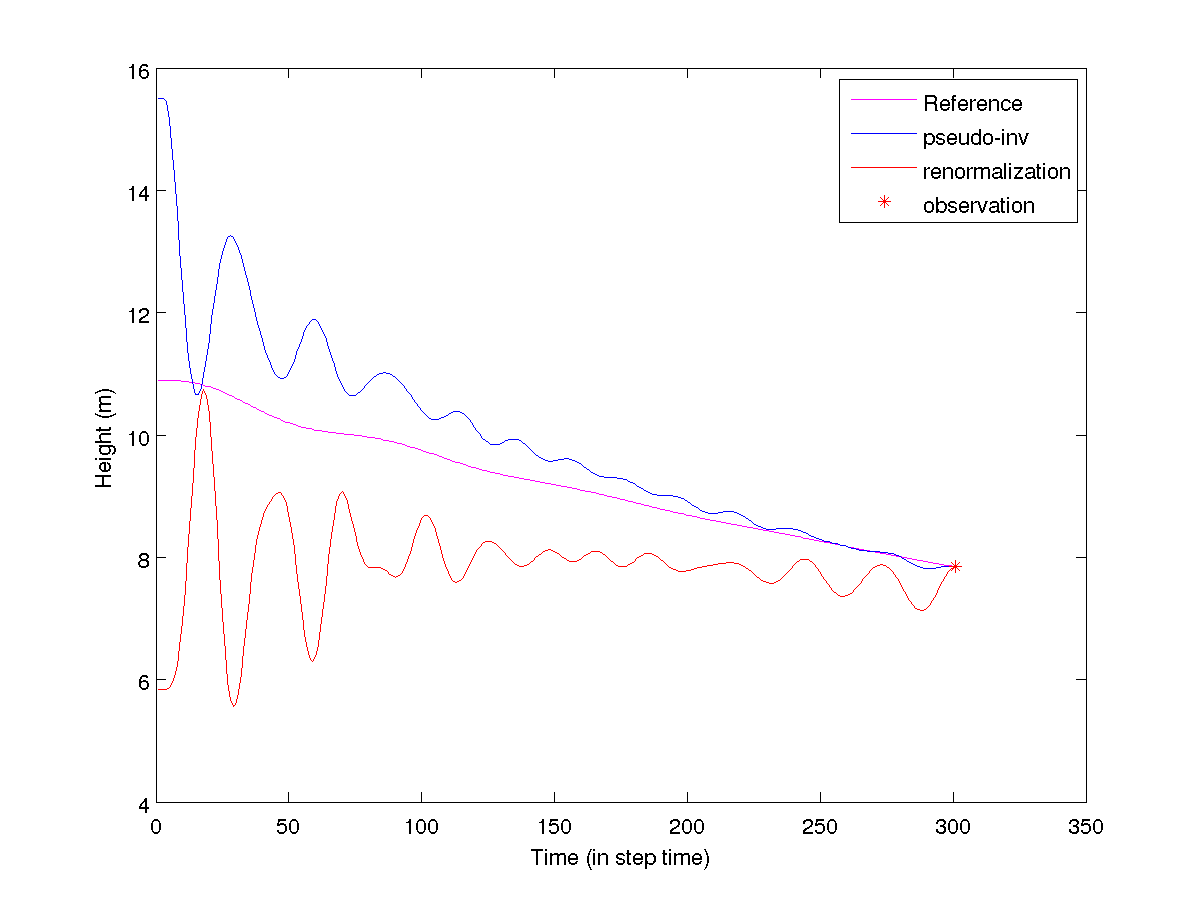
\includegraphics[scale=0.55]{./fig/121obs/compare_sol.png}
\end{figure}
\end{frame}

\begin{frame}
\frametitle{Ecart à la référence}
\begin{figure}
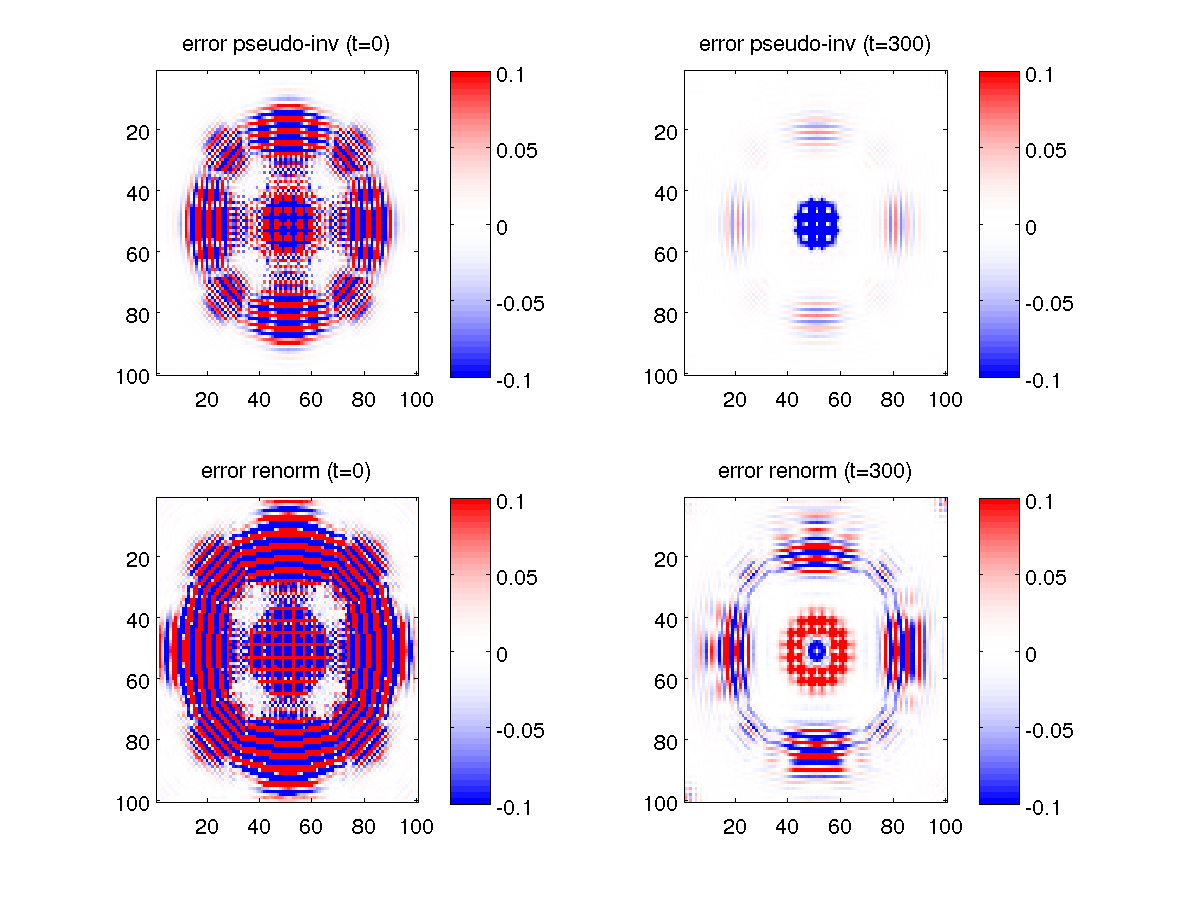
\includegraphics[scale=0.55]{./fig/121obs/error_H.png}
\end{figure}
\end{frame}

\begin{frame}
\frametitle{Résulats pour le paramètre U  (pseudo-inverse)}
\begin{figure}
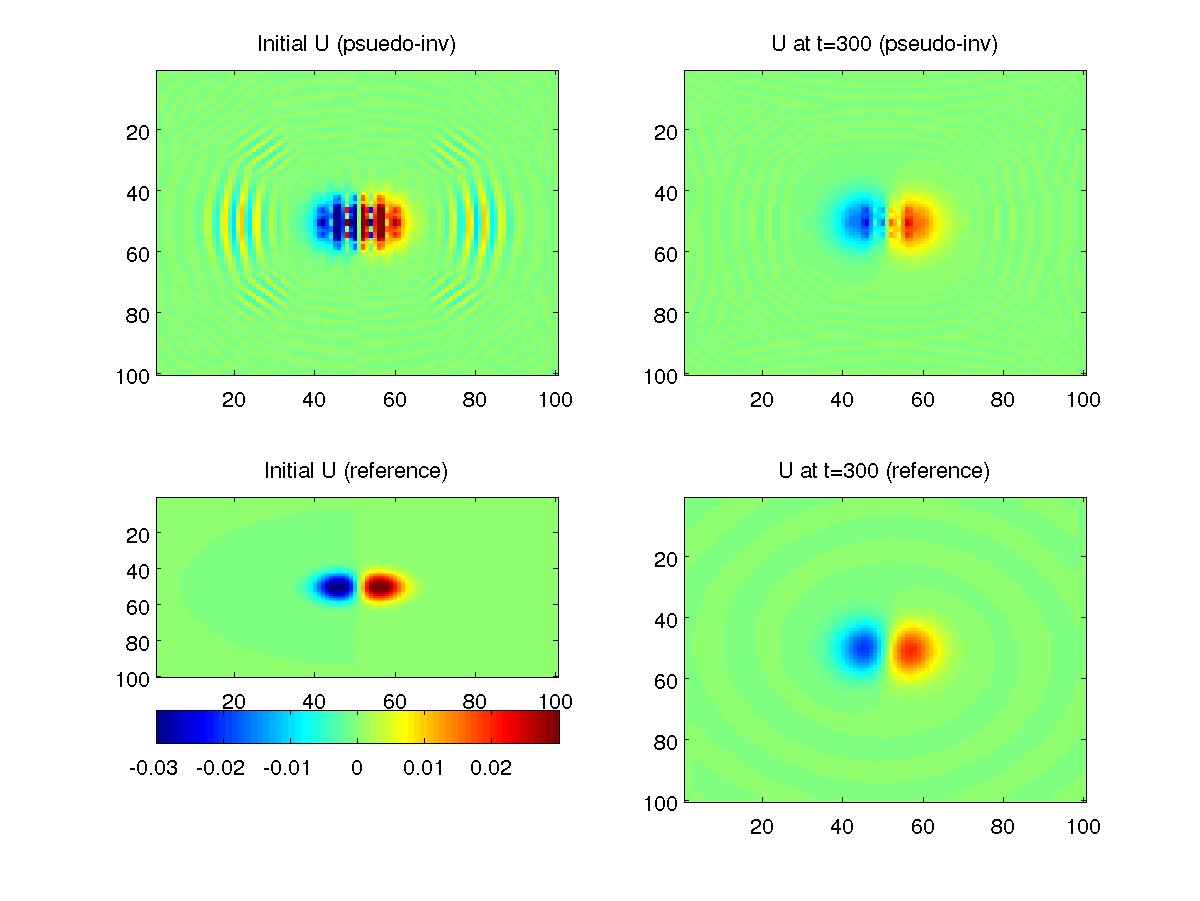
\includegraphics[scale=0.55]{./fig/121obs/pseudoinv-sol-U.png}
\end{figure}
\end{frame}

\begin{frame}
\frametitle{Résulats pour le paramètre U  (renormalisation)}
\begin{figure}
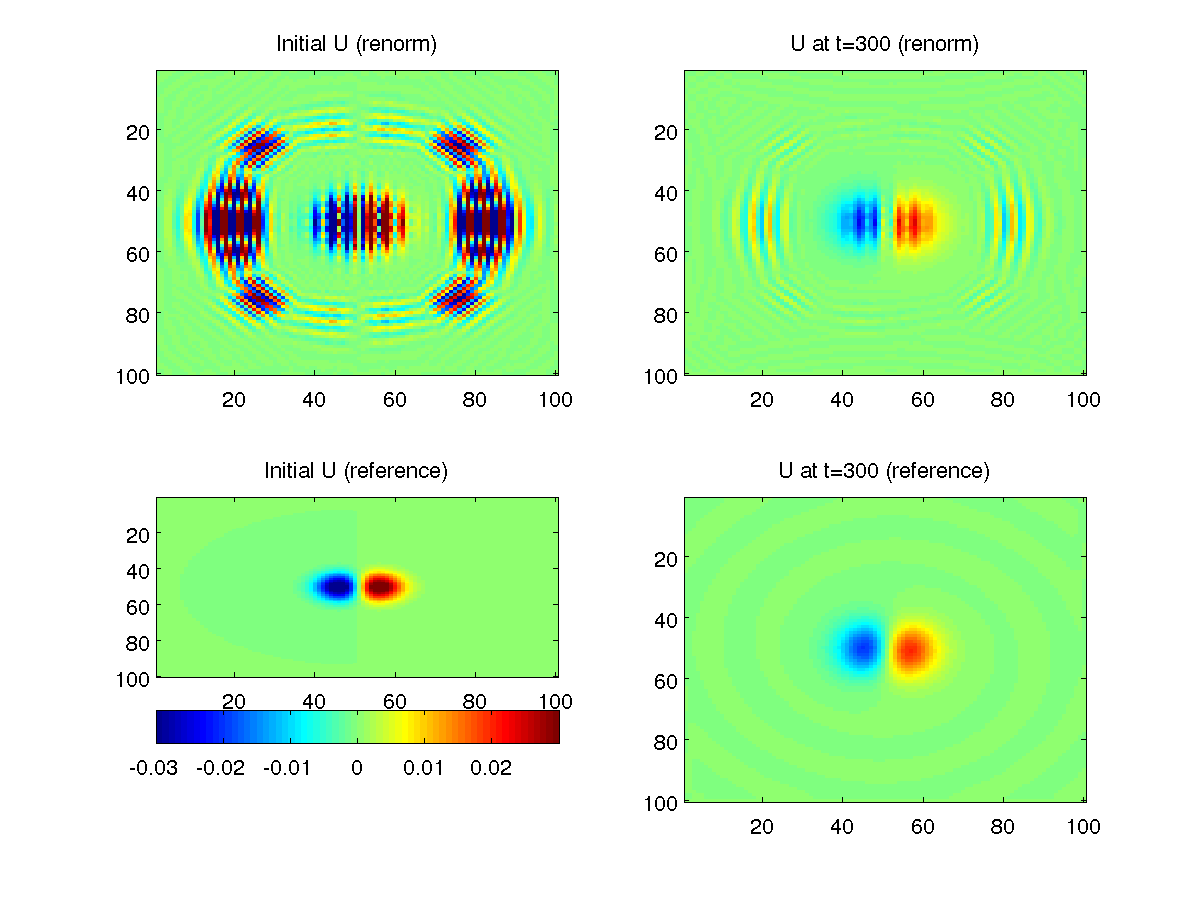
\includegraphics[scale=0.55]{./fig/121obs/renorm-sol-U.png}
\end{figure}
\end{frame}

\begin{frame}
\frametitle{Conclusion}
\begin{itemize}
\item Problème du schéma numérique (si le champ est trop irrégulier).\\
\item Corriger l'instant initial pour $u$ et $v$ aussi afin de retrouver une plus grande variété de conditions initiales.\\
\item Aller vers le non-linéaire.\\
\end{itemize}
\end{frame}


%%%%%% SECTION 12
%\include{algorithmes}
\end{document}


%%%%%%%%%%%%%%%%%%%%% SECTION 1
\section{Les algorithmes}\label{section:1}
\begin{frame}
\begin{columns}
        \column{4.8cm}
            \tableofcontents[currentsection]
        \column{7cm}
        \centering{
            \includegraphics[width=7cm]{fig/Algorithm-sheldon.png}
            
                 \textit{ I believe I've isolateblblblblblblsblbslbslbsl
            sblbslblsblsblblsblbs
            lbslblbslsb d the algorithm for making friends.}
     
            
            \small{
            \hfill Sheldon Cooper, 
            
            \hfill in \textit{The Big Band Theory}, Season 2, Episode 13
            }
}

    \end{columns}

\end{frame}


%%%%%%%%%%%%%%%%%%%%%
\subsection{Introduction}
    \begin{frame}
    \frametitle{Pourquoi faire appel à des algorithmes ?}
    Pour automatiser des tâches
    
    Exemples :
    \begin{itemize}
    \item Métier à tisser\\
    \item Méthode de calcul à la main d'une division\\
    \item Recette de cuisine\\
    \item ...\\
    \end{itemize}
    \end{frame}
 
 %%%%%%%%%%%%%%%%%
 
    \begin{frame}
    \frametitle{Qu'est-ce qu'un algorithme ?}
    \begin{block}{Définition}
    Un algorithme est un ensemble 
    ordonné d'instructions simples
permettant de résoudre un problème.
    \end{block}
    \end{frame}
    
 %%%%%%%%%%%%%%%%%%
 \subsection{Construction d'un algorithme}
%%%%%%%%%%%%%%%%%%%    
\section{La machine de Turing}
%%%%%%%%%%%%%%%%%%%%
 
  
\begin{frame}[fragile]
\frametitle{Un peu d'histoire...}
\begin{codeblock}{Test}
\begin{codeC}
for (int i = 0 ; i < n ; i ++) {
    //a comment
    printf("%d",i);
    }
\end{codeC}
\end{codeblock}

\begin{termblock}{test 2}
\lstset{escapeinside={§§}}
\begin{lstlisting}
§\textbf{>>}§./a.out
§\color{darkgray}{\texttt{  Hello World}}§
\end{lstlisting}
\end{termblock}

 \begin{block}{Bloc standard}
blablabla
\end{block}
\end{frame}


\begin{frame}[fragile]
\frametitle{essai}
\begin{columns}
\column{6cm}
\begin{block}

\begin{figure}
\begin{tikzpicture} [
    auto,
    decision/.style = { diamond, draw=blue, thick, fill=blue!20,
                        text width=5em, text badly centered,
                        inner sep=1pt, rounded corners },
    block/.style    = { rectangle, draw=blue, thick, 
                        fill=blue!20, text width=10em, text centered,
                        rounded corners, minimum height=2em },
    line/.style     = { draw, thick, ->, shorten >=2pt },
  ]
   \matrix [column sep=-10mm, row sep=10mm] {
                    & \node [text centered] (x) {$\mathbf{X}$};            & \\
                    & \node (null1) {};                                    & \\
                    & \node [block] (doa) {\textsf{DoAE}($\mathbf{X}$)};   & \\
  	               \node(null3){}; & \node [decision] (uiddes)
                        {\textsf{UID}($\hat{\mathbf{X}}$)};
                                  & \node[text centered](tra){$\mathbf{i}$}; \\
                  & \node [block] (track) {\textsf{DoAT}($\mathbf{x}$)}; & \\
                    & \node [block] (pesos)
                        {\textsf{BF}(DoA$_{\mathrm{T}}$,DoAs)};            & \\
                    & \node [block] (filtrado)
                        {\textsf{SF}($\mathbf{w}$,$\mathbf{x}$)};          & \\
                    & \node [text centered] (xf) {$\hat{x}(t)$ };          & \\
  };
  % connect all nodes defined above
 \begin{scope} [every path/.style=line]
    \path (x)        --    (doa);
    \path (doa)      --    node [near start] {DoAs} (uiddes);
    \path (tra)      --    (uiddes);
    \path (uiddes)   --++  (-3,0) node [near start] {no} |- (null1);
    \path (uiddes)   --    node [near start] {DoA} (track);
    \path (track)    --    node [near start] {DoA$_{\mathrm{T}}$} (pesos);
    \path (pesos)    --    node [near start] {\textbf{w}} (filtrado);
    \path (filtrado) --    (xf);
  
  \end{scope}
\end{tikzpicture}
\end{figure}
\end{block}
\column{3cm}
\begin{block}{bulbul}
\end{block}
\end{columns}
\end{frame}

\end{document}
